% Convolutional Autoencoder
% Modified Version Of: https://github.com/jettan/tikz_cnn

\newcommand{\CaeImgHeight}{25mm}%
% Source: https://tex.stackexchange.com/questions/295100/partial-or-entire-image-blurring-in-tikz
%Parameters:
%- at position
%- blur parameter
%- image name
\newcommand\blurredimage[3]{%
  \node[opacity=1.0] (output image) at (#1) {\includegraphics[height=\CaeImgHeight]{#3}};
  \node[opacity=0.2] at (#1+ #2, #2) {\includegraphics[height=\CaeImgHeight]{#3}};
  \node[opacity=0.2] at (#1+-#2, #2) {\includegraphics[height=\CaeImgHeight]{#3}};
  \node[opacity=0.2] at (#1+-#2,-#2) {\includegraphics[height=\CaeImgHeight]{#3}};
  \node[opacity=0.2] at (#1+ #2,-#2) {\includegraphics[height=\CaeImgHeight]{#3}};
}%


\centering
\hspace{9in}\resizebox{\textwidth}{!}{%
  \begin{tikzpicture}%
    \draw[use as bounding box, transparent] (-1.8,-1.8) rectangle (17.2, 3.2);
    % Define the macro.
    % 1st argument: Height and width of the layer rectangle slice.
    % 2nd argument: Depth of the layer slice
    % 3rd argument: X Offset --> use it to offset layers from previously drawn layers.
    % 4th argument: Options for filldraw.
    % 5th argument: Text to be placed below this layer.
    % 6th argument: Y Offset --> Use it when an output needs to be fed to multiple layers that are on the same X offset.
    \newcommand{\networkLayer}[6]{%
      \def\a{#1} % Used to distinguish input resolution for current layer.
      \def\b{0.02} %
      \def\c{#2} % Width of the cube to distinguish number of input channels for current layer.
      \def\t{#3} % X offset for current layer.
      \def\d{#4} % Y offset for current layer.
      % Draw the layer body.
      \draw[line width=0.3mm](\c+\t,0,\d) -- (\c+\t,\a,\d) -- (\t,\a,\d);              % back plane
      \draw[line width=0.3mm](\t,0,\a+\d) -- (\c+\t,0,\a+\d) node[midway,below] {#6} -- (\c+\t,\a,\a+\d) -- (\t,\a,\a+\d) -- (\t,0,\a+\d); % front plane
      \draw[line width=0.3mm](\c+\t,0,\d) -- (\c+\t,0,\a+\d);
      \draw[line width=0.3mm](\c+\t,\a,\d) -- (\c+\t,\a,\a+\d);
      \draw[line width=0.3mm](\t,\a,\d) -- (\t,\a,\a+\d);
      % Recolor visible surfaces
      \filldraw[#5] (\t+\b,\b,\a+\d) -- (\c+\t-\b,\b,\a+\d) -- (\c+\t-\b,\a-\b,\a+\d) -- (\t+\b,\a-\b,\a+\d) -- (\t+\b,\b,\a+\d); % front plane
      \filldraw[#5] (\t+\b,\a,\a-\b+\d) -- (\c+\t-\b,\a,\a-\b+\d) -- (\c+\t-\b,\a,\b+\d) -- (\t+\b,\a,\b+\d);
      % Colored slice.
      \ifthenelse {\equal{#5} {}} %
      {} % Do not draw colored slice if #4 is blank.
      {\filldraw[#5] (\c+\t,\b,\a-\b+\d) -- (\c+\t,\b,\b+\d) -- (\c+\t,\a-\b,\b+\d) -- (\c+\t,\a-\b,\a-\b+\d);} % Else, draw a colored slice.
    } %
    \begin{scope}[shift={(5,0)}]
      \onslide<+->{
        % INPUT
        \node[] (input image) at (-3.75,0.5) {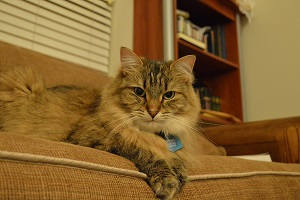
\includegraphics[height=\CaeImgHeight]{tikz/img/muffins.jpg}};
        \node[above of=input image, node distance=1.8cm] {\LARGE $\mathbf{x}$};
        \networkLayer{3.0}{0.03}{-0.5}{0.0}{color=gray!80}{} %
        % ENCODER
        \networkLayer{3.0}{0.1}{0.0}{0.0}{color=white}{}    %
        \networkLayer{2.5}{0.2}{0.4}{0.0}{color=white}{}    %
        \networkLayer{2.0}{0.4}{0.95}{0.0}{color=white}{}   %
        \networkLayer{1.5}{0.4}{1.5}{0.0}{color=white}{}    %
        % BOTTLENECK
        \networkLayer{1.0}{0.4}{2.3}{0.0}{color=red!40}{}    %
        % DECODER
        \networkLayer{1.5}{0.4}{3.3}{0.0}{color=white}{}    %
        \networkLayer{2.0}{0.4}{4.3}{0.0}{color=white}{}    %
        \networkLayer{2.5}{0.2}{5.3}{0.0}{color=white}{}    %
        \networkLayer{3.0}{0.1}{6.2}{0.0}{color=white}{}    %
        % OUTPUT
        \networkLayer{3.0}{0.05}{7.2}{0.0}{color=blue!20}{}  %
        \blurredimage{8.9,0.5}{0.10}{tikz/img/muffins.jpg}  %
        \node[above of=output image, node distance=1.8cm] {\LARGE $\mathbf{\hat{x}}$};
      }
      \onslide<+->{%
        \draw[dashed, blue, thick] (-1.8,3.4) rectangle (2.8,-1.5);
        \node[] () at (-0.3, 3.8) {\blue{\textbf{Encoder}}};
      }
      \onslide<+->{%
        \draw[dashed, color=dartmouthgreen, thick] (1.8,3.4) rectangle (7.5,-1.5);
        \node[] () at (5.4, 3.8) {\textbf{\color{dartmouthgreen} Decoder}};
      }
      \onslide<+->{%
        \draw[color=lust, thick] (1.8,3.4) rectangle (2.8,-1.5);
        \node[] () at (2.3, 3.8) {\textbf{\color{lust} Bottleneck}};
      }
    \end{scope}
  \end{tikzpicture}  %
}
